\subsection{Parameter Effects}
\label{sec:setup.char.paramfx}

%\todo{
%	Automatische Übersetzung meiner e-mail. Leicht, aber nur leicht, nachbearbeitet :-)
%	Es ist noch kein Englisch, aber es ist bereits lesbar.
%
%	1) Mapping a circle onto itself.
%	Well it's just because we we are talking about a phase, there is no need to prove anything. It is probably trivial as well to show that the function has no fixed points, that is, F(x)>x mod 2 pi, right?
%
%	2a) The function is discontinuous. Disc. points are caused by tangencies...etc.
%	It is not particularly necessary to calculate these disc. points analytically as we do not use analytical expressions further.
%
%	2b) Which would be really cool, but I'm not sure how realistic it is - explain why, in a given range of parameters, the obtained function has exactly four disc. points.
%
%	3) Contractive function: here, theoretically, it is possible write the derivative dF/dx and show that it is less in absolute value units, but there are eight implicit functions, I really don’t want to. If there is a physical explanation why it should work this way - great, if not, and okay, it's enough to say what can be calculated and shown.
%
%	4) Symmetry F(x+pi)=F(x)+pi, where does it come from. I would say that the perfect explanation I can imagine is schematic picture. Why exactly trajectories for initial conditions lagging behind each other by half a period, after one step come to points that are half a period behind each other.
%
%	5a) Minimum points - where do they come from. In the last article this was discussed, the same thing here - draw a trajectory with a tangency from some initial condition and two neighboring trajectories, coming both to the same point a little later than the first one. And that's it, plus a couple of lines of text.
%
%	5b) But then everything becomes more complicated. Since we already talked about symmetry, it is enough to talk about the first two branches. We also said for the minimums where they come from. Question: is it possible show (again, schematically!) that these minimum points are within corresponding domains of the branches? This is less important for the first part of the article, but for the second one it is fundamental: what does it mean if the minimum point moves to the edge of the branch and goes beyond it. If it's at all possible, I don't know.
%}

In this section, we examine the effects of the parameters on the original model function.
We start with the combined parameter effects along a chain of parameter regions of the same period.
After that we will look into what role the parameters play individually.

\subsection{Combined Effects of Parameters}
\label{sec:setup.char.paramfx.combined}
\label{sec:yunus.param.effects.combined}

To replicate the dynamics seen in the model, it is helpful to know, how the model changes along the areas of the same period.
\Cref{fig:setup.char.evolution.12} shows, how the model function changes along the area of period 12.
In the figure, there are three functions in three different colors.
The first function is blue, and it is the model with parameters $E_0 = 15.9, \chi_0 = 0.11$, it is marked as point $A_12$ in \Cref{fig:setup.char.evolution.map}.
The second function is purple, and it is the model at the point $E_0 = 17.07, \chi_0 = 0.182$, marked as point $B_{12}$.
The last function is red, and it is the model with parameters $E_0 = 18.5, \chi_0 = 0.27$, marked as point $C_{12}$.

\begin{figure}
	\centering
	\begin{subfigure}{0.4\textwidth}
		\includegraphics[width=\textwidth]{99_Yunus/2D_Period_Zoomed_Effects/result.png}
		\caption{Points}
		\label{fig:setup.char.evolution.map}
	\end{subfigure}
	\begin{subfigure}{0.4\textwidth}
		\includegraphics[width=\textwidth]{99_Yunus/ParameterEffects/E0_hi_P12/illustration.png}
		\caption{Period 12}
		\label{fig:setup.char.evolution.12}
	\end{subfigure}
	\begin{subfigure}{0.4\textwidth}
		\includegraphics[width=\textwidth]{99_Yunus/ParameterEffects/E0_hi_P10/illustration.png}
		\caption{Period 10}
		\label{fig:setup.char.evolution.10}
	\end{subfigure}
	\begin{subfigure}{0.4\textwidth}
		\includegraphics[width=\textwidth]{99_Yunus/ParameterEffects/E0_hi_P08/illustration.png}
		\caption{Period 8}
		\label{fig:setup.char.evolution.08}
	\end{subfigure}
	\caption[Effects of parameters on the original model function]{
		The shapes of the original model function for different parameter values.
		(a) shows the points of the parameter values used for the other figures.
		(b) shows the evolution of the shape of the original model function along the chain of parameter regions with period 12 cycles.
		The blue function is the model function for the parameter values at point $A_{12}$, purple at point $B_{12}$, and red at point $C_{12}$.
		Here, blue is at point $A_{10}$, purple at point $B_{10}$, and red at point $C_{10}$.
		(c) shows the same thing for the chain of parameter regions with period 10.
		And (d) is for the chain of parameter regions with period 8.
		Here, blue is at point $B_8$ and red at point $C_8$.
	}
	\label{fig:setup.char.evolution.combined}
\end{figure}

The most notable changes are
\begin{enumerate*}
	\item The values of branches $f_\A$ and $f_\C$ get larger while the values at the left borders get larger more
	\item The value at the left borders of branches $f_\B$ and $f_\D$ get smaller
	\item The local minima of these branches move left, and their values get smaller.
\end{enumerate*}
One smaller change is that the border between branches $\B$ and $\C$ moves left.
Note that the same change happens to the border between the branches $\D$ and $\A$ due to the symmetry of the function.

The same effects can be observed for the areas of period 8 and 10.
The effects are visualized in \Cref{fig:setup.char.evolution.10,fig:setup.char.evolution.08}.
The points used for measurement are visualized in \Cref{fig:setup.char.evolution.map}.
For the period 10, points $A_{10}, B_{10},$ and $C_{10}$ are used and for period 8, points $B_8$ and $C_8$.

\subsection{Individual Effects of Parameters}
\label{sec:yunus.param.effects.individual}

The effects of the parameters described above, always include a change in both parameters $E_0$ and $\chi_0$.
To reproduce the bifurcation structures, it is important to know which effects on the function each parameter has individually.

\begin{figure}
	\centering
	\includegraphics[width=0.4\textwidth]{99_Yunus/2D_Period_Zoomed_EffectsSingle/result.png}
	\caption[The parameter ranges examined to analyze the effects of parameters on the original model function]{
		The parameter ranges examined to analyze the effects of parameters $E_0$ and $\chi_0$ on the original model function
		The green arrow indicates the parameter range used for analyzing the effects of the parameter $E_0$, while the orange arrow indicates the parameter range used for analyzing the effects of the parameter $\chi_0$ on the original model function.
	}
	\label{fig:setup.char.evolution.single.map}
\end{figure}

For the parameter $E_0$, we fixed $\chi_0 = 0.2$ and varied $E_0$ in the parameter range $[15, 19]$, it is marked as the green arrow in \Cref{fig:setup.char.evolution.single.map}.
Like before, we took the function at three points and put them in one figure with color codes.
This is illustrated in \Cref{fig:setup.char.evolution.e0}.
The blue function is the function of the original model at the start of the parameter range, $E_0 = 15$ and $\chi_0 = 0.2$.
The purple function is in the middle at $E_0 = 17$ and $\chi_0$ stays the same.
And the red function is at the end at $E_0 = 19$.
From the figure we can see three effects, the parameter has on the function of the original model in this parameter range.
The observed changes are
\begin{enumerate*}
	\item The values at the left border of branches $f_\B$ and $f_\D$ get smaller
	\item The local minima of these branches move to the left and their values get smaller
	\item The border between branches $f_\A$ and $f_\B$ moves right (so does the border between branches $f_\C$ and $f_\D$)
	\item The values at the right borders of branches $f_\A$ and $f_\C$ get larger (This is caused by the border between branches $f_\A$ and $f_B$ moving right).
\end{enumerate*}

For the parameter $\chi_0$, we fixed $E_0 = 17$ and varied $\chi_0$ in the parameter range $[0.125, 0.3]$.
This parameter range is marked orange in \Cref{fig:setup.char.evolution.single.map}.
The function is displayed at three points of the parameter range in \Cref{fig:setup.char.evolution.hi}.
As before, the blue function is the function of the original model at the start of the parameter range, $E_0 = 17$ and $\chi_0 = 0.125$.
The purple function is at $\chi_0 = 0.2125$, and the red one is at $\chi_0 = 0.3$.
The observed changes are
\begin{enumerate*}
	\item The values of the branches $f_\A$ and $f_\C$ get larger
	\item The border between the branches $f_\A$ and $f_\B$ moves left (so does the border between branches $f_\C$ and $f_\D$).
\end{enumerate*}
Two more changes are smaller in comparison
\begin{enumerate*}
	\item The values at the right borders of the branches $f_\B$ and $f_\D$ get larger (including the minima)
	\item The border between the branches $f_\B$ and $f_\C$ moves left (so does the border between branches $f_\D$ and $f_\A$).
\end{enumerate*}

\begin{figure}
	\centering
	\begin{subfigure}{0.4\textwidth}
		\includegraphics[width=\textwidth]{99_Yunus/ParameterEffects/E0/illustration.png}
		\caption{Parameter $E_0$}
		\label{fig:setup.char.evolution.e0}
	\end{subfigure}
	\begin{subfigure}{0.4\textwidth}
		\includegraphics[width=\textwidth]{99_Yunus/ParameterEffects/hi/illustration.png}
		\caption{Parameter $\chi_0$}
		\label{fig:setup.char.evolution.hi}
	\end{subfigure}
	\caption[The effects of single parameters on the original model function]{
		The effects of varying the parameters $E_0$ and $\chi_0$ alone on the original model function.
		(a) shows the effects of $E_0$ on the original model function.
		The red function is at the beginning of the parameter range depicted in \Cref{fig:setup.char.evolution.single.map}, purple is in the middle, and red is at the end.
		(b) shows the effects of $\chi_0$ on the original model function.
		Analogously to (a), the red function is at the beginning of the parameter range depicted in \Cref{fig:setup.char.evolution.single.map}, purple is in the middle, and red is at the end.
	}
	\label{fig:setup.char.evolution.single}
\end{figure}

\subsection{Decomposition of Combined Effects}
\label{sec:yunus.param.effects.decomposition}

Now we can take a closer look at the combined effects of the parameters along areas of the same period and trace them back to the isolated effects of both parameters.
For this, we introduce a notation for the effects.
The effect of the values at the left border of a branch changing is denoted $\AL$, for the right border $\AR$, and for the whole branch $\AW$
The subscript indicates, which branch the change effects, and the superscript indicates, whether the values get larger $+$ or smaller $-$.
The effect of changing a local minimum is denoted as $\AMi$.
The meaning of the subscript stays the same as above, but the superscript also can include $L$ for left movement and $R$ for right movement.
Finally, the effect of moving borders is denoted as $\AB$.
The subscript now includes the two branches, to which the border belongs, and the superscript now has only $L$ or $R$.
For brevity, we do not write redundant branch names, so changes happening to branch $\A$ are also happening to branch $\C$.
For borders, changes to the border between branches $\A$ and $\B$ are also happening to the border between branches $\C$ and $\D$ and so on.

\Cref{tab:yunus.parameter.effects} lists all observed effects along the areas of the same period and their decomposition into effects of the single parameters.
The first part of the table includes all major changes observed in \Cref{sec:yunus.param.effects.combined}, while the second part focuses on the minor change.
The second part also includes the changes observed in \Cref{sec:yunus.param.effects.individual} that cancel out.
From this table we can see, that $E_0$ causes the effects on the branches $\B$ and $\D$, while $\chi_0$ causes the changes to the branches $\A$ and $\C$, as well as the minor movement of the borders between branches $\B$ and $\C$.
Note again, that the change to the border of branches $\B$ and $\C$ also applies for the border between branches $\D$ and $\A$.

\begin{table}
	\centering
	\begin{tabular}{|c|c|c|l|} \hline
		Combined         & $E_0$            & $\chi_0$          & Comment                   \\ \hline \hline
		$\AL_{\B}^{-}$   & $\AL_{\B}^{-}$   & 0                 & Only $E_0$ causes this    \\ \hline
		$\AMi_{\B}^{L-}$ & $\AMi_{\B}^{L-}$ & $-\AMi_{\B}^{+}$  &
		$E_0$ and $\chi_0$ have opposing effects, the effect of $E_0$ is stronger           \\ \hline
		$\AW_{\A}^{+}$   & 0                & $\AW_{\A}^{+}$    & Only $\chi_0$ causes this \\ \hline \hline
		$\AB_{\B\C}^{L}$ & 0                & $\AB_{\B\C}^{L}$  & Only $\chi_0$ causes this \\ \hline
		0                & $\AB_{\A\B}^{R}$ & $-\AB_{\A\B}^{L}$ &
		$E_0$ and $\chi_0$ have opposing effects, they cancel out                           \\ \hline
	\end{tabular}
	\caption[Decomposition table of combined parameter effects]{
		Decomposition of the combined parameter effects along chains of parameter regions with the same period as displayed in \Cref{fig:setup.char.evolution.combined}.
		Each effect is traced back to the effects of changing the parameters $E_0$ and $\chi_0$ alone as displayed in  \Cref{fig:setup.char.evolution.single}.
	}
	\label{table:setup.char.paramfx}
\end{table}
